\documentclass[12pt,a4paper]{article}

\usepackage[utf8]{inputenc}
\usepackage[T1]{fontenc}
\usepackage[english]{babel}
\usepackage{amsmath, amssymb, amsthm}
\usepackage{geometry}
\usepackage{booktabs}
\usepackage{hyperref}
\usepackage{parskip}
\usepackage{tikz}
\usetikzlibrary{arrows.meta, calc}

\geometry{margin=2.5cm}

\hypersetup{
    colorlinks=true,
    linkcolor=blue!60!black,
    urlcolor=blue!60!black,
}

\title{\textbf{Evaluación de Integrales de Dominio mediante Dual Reciprocity}\\[0.5em]
\large Ejemplo: Dominio Circular\\[0.3em]
\normalsize Notas para un Curso de Maestría en Boundary Element Method}
\author{W.F. Florez\\
\small Wessex Institute of Technology}
\date{}

\begin{document}

\maketitle
\tableofcontents
\newpage

% ─────────────────────────────────────────────────────────────
\section{Planteamiento del Problema}
% ─────────────────────────────────────────────────────────────

Se desea evaluar la integral de dominio

\begin{equation}
    I = \int_\Omega b(x,y)\, d\Omega
\end{equation}

sobre el disco circular de radio $R$:

\begin{equation}
    \Omega = \left\{ (x,y) \in \mathbb{R}^2 : x^2 + y^2 \leq R^2 \right\}
\end{equation}

con la función:

\begin{equation}
    b(x,y) = x^2 + y^2
\end{equation}

\subsection{Solución Analítica}

Pasando a coordenadas polares $(x,y) = (\rho\cos\theta,\, \rho\sin\theta)$
con $d\Omega = \rho\,d\rho\,d\theta$:

\begin{equation}
    I = \int_0^{2\pi}\int_0^R \rho^2 \cdot \rho\, d\rho\, d\theta
      = 2\pi \int_0^R \rho^3\, d\rho
      = 2\pi \cdot \frac{R^4}{4}
      = \frac{\pi R^4}{2}
\end{equation}

Para $R = 1$:

\begin{equation}
    I_{\text{exacta}} = \frac{\pi}{2} \approx 1.5707963268
\end{equation}

\subsection{Motivación para el Dominio Circular}

El disco circular presenta ventajas pedagógicas concretas respecto al
cuadrado estudiado anteriormente:

\begin{enumerate}
    \item \textbf{Parametrización exacta de $\Gamma$:} la frontera se
    parametriza como $\mathbf{x}(t) = (R\cos t,\, R\sin t)$, $t\in[0,2\pi]$,
    con normal exterior exactamente $\mathbf{n} = (\cos t,\, \sin t)$.

    \item \textbf{Error geométrico visible:} con elementos constantes
    (cuerdas), la geometría circular se aproxima y aparece un error
    geométrico que antes era nulo en el cuadrado. Esto permite separar
    conceptualmente el error geométrico del error de interpolación RBF.

    \item \textbf{Distribución polar de nodos:} los nodos de colocación
    internos se distribuyen naturalmente en coordenadas polares, introduciendo
    la cuestión de la distribución óptima de puntos como tema de discusión.

    \item \textbf{Convergencia no monótona instructiva:} si se refina solo la
    malla de contorno manteniendo fijos los nodos de colocación, el error
    no decrece monótonamente, revelando la interacción entre las dos fuentes
    de error.
\end{enumerate}

% ─────────────────────────────────────────────────────────────
\section{Formulación DR para el Dominio Circular}
% ─────────────────────────────────────────────────────────────

\subsection{Recordatorio: Conversión de Integral de Dominio}

De acuerdo con la formulación desarrollada previamente, la integral de
dominio se convierte en integrales de frontera mediante:

\begin{equation}
    I \approx \sum_{j=1}^{N} \alpha_j \int_\Gamma
    \frac{\partial\hat{\phi}_j}{\partial n}\, d\Gamma_x
\end{equation}

donde los coeficientes $\boldsymbol{\alpha} = \mathbf{F}^{-1}\mathbf{b}$
se obtienen por colocación RBF, y la función particular $\hat{\phi}_j$
satisface $\nabla^2\hat{\phi}_j = f_j(r_j)$.

\subsection{RBF y Función Particular}

Se utiliza:

\begin{equation}
    f(r) = 1 + r^3 \implies
    \hat{\phi}(r) = \frac{r^2}{4} + \frac{r^5}{25}, \qquad
    \frac{d\hat{\phi}}{dr} = \frac{r}{2} + \frac{r^4}{5}
\end{equation}

y la derivada normal:

\begin{equation}
    \frac{\partial\hat{\phi}_j}{\partial n}
    = \left(\frac{1}{2} + \frac{r_j^3}{5}\right)
    (\mathbf{x} - \mathbf{x}_j)\cdot\mathbf{n}
\end{equation}

% ─────────────────────────────────────────────────────────────
\section{Geometría: Elementos Constantes sobre el Círculo}
% ─────────────────────────────────────────────────────────────

\subsection{Parametrización de los Elementos}

Se divide $\Gamma$ en $N_e$ elementos rectos (cuerdas). Los nodos extremos
del elemento $k$ se obtienen de:

\begin{equation}
    \theta_k = \frac{2\pi k}{N_e}, \quad k = 0, 1, \ldots, N_e
\end{equation}

\begin{equation}
    \mathbf{x}_k^1 = \begin{pmatrix} R\cos\theta_k \\ R\sin\theta_k \end{pmatrix},
    \qquad
    \mathbf{x}_k^2 = \begin{pmatrix} R\cos\theta_{k+1} \\ R\sin\theta_{k+1} \end{pmatrix}
\end{equation}

La parametrización local con $t\in[-1,1]$:

\begin{equation}
    \mathbf{x}(t) = \frac{1-t}{2}\mathbf{x}_k^1 + \frac{1+t}{2}\mathbf{x}_k^2
\end{equation}

\subsection{Normal Exterior y Jacobiano}

El vector tangente de la cuerda es constante en cada elemento:

\begin{equation}
    \mathbf{T}_k = \mathbf{x}_k^2 - \mathbf{x}_k^1
    = \begin{pmatrix} \Delta x_k \\ \Delta y_k \end{pmatrix},
    \qquad L_k = \|\mathbf{T}_k\|
\end{equation}

La normal exterior unitaria (perpendicular a la cuerda, apuntando hacia afuera):

\begin{equation}
    \mathbf{n}_k = \frac{1}{L_k}
    \begin{pmatrix} \Delta y_k \\ -\Delta x_k \end{pmatrix}
\end{equation}

El jacobiano de la transformación $t\in[-1,1]$:

\begin{equation}
    J_k = \frac{L_k}{2}
\end{equation}

\subsection{Error Geométrico de la Aproximación por Cuerdas}

Con elementos constantes, la longitud real del arco del elemento $k$ es
$\ell_k = R\,\Delta\theta = 2\pi R/N_e$, mientras que la longitud de la
cuerda es:

\begin{equation}
    L_k = 2R\sin\!\left(\frac{\pi}{N_e}\right)
\end{equation}

El error geométrico relativo por elemento es:

\begin{equation}
    \varepsilon_{\text{geom}} = 1 - \frac{L_k}{\ell_k}
    = 1 - \frac{N_e}{\pi}\sin\!\left(\frac{\pi}{N_e}\right)
    \approx \frac{\pi^2}{6N_e^2} \quad (N_e \gg 1)
\end{equation}

Este error es $O(N_e^{-2})$, lo que fija la tasa de convergencia geométrica
independientemente de la calidad de la interpolación RBF.

\begin{figure}[h]
\centering
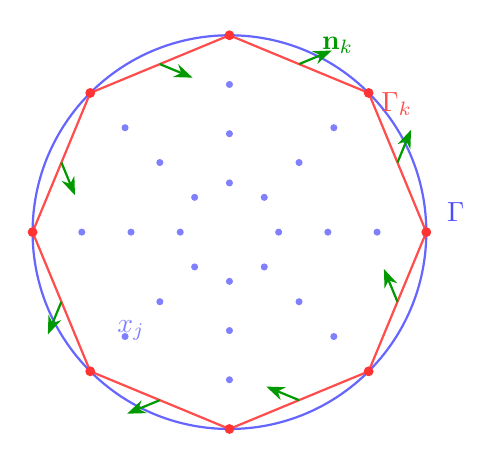
\begin{tikzpicture}[scale=2.5]
    % Circulo exacto
    \draw[blue!60, thick] (0,0) circle (1);
    % 8 cuerdas
    \foreach \k in {0,...,7} {
        \draw[red!70, thick]
            ({cos(\k*45)},{sin(\k*45)}) --
            ({cos(\k*45+45)},{sin(\k*45+45)});
    }
    % Nodos extremos
    \foreach \k in {0,...,7} {
        \fill[red!80] ({cos(\k*45)},{sin(\k*45)}) circle (0.025);
    }
    % Normales en cada elemento (mitad de la cuerda)
    \foreach \k in {0,...,7} {
        \pgfmathsetmacro{\ax}{0.5*(cos(\k*45)+cos(\k*45+45))}
        \pgfmathsetmacro{\ay}{0.5*(sin(\k*45)+sin(\k*45+45))}
        \pgfmathsetmacro{\nx}{sin(\k*45+22.5)}
        \pgfmathsetmacro{\ny}{-cos(\k*45+22.5)*(-1)}
        \draw[-{Stealth}, green!60!black, thick]
            (\ax,\ay) -- ({\ax+0.18*\nx},{\ay+0.18*\ny});
    }
    % Nodos de colocacion internos (ejemplo esquematico)
    \foreach \ring in {1,2,3} {
        \foreach \ang in {0,45,...,315} {
            \fill[blue!50]
                ({0.25*\ring*cos(\ang)},{0.25*\ring*sin(\ang)}) circle (0.018);
        }
    }
    % Etiquetas
    \node[blue!70] at (1.15, 0.1) {$\Gamma$};
    \node[red!70]  at (0.85, 0.65) {$\Gamma_k$};
    \node[green!60!black] at (0.55, 0.95) {$\mathbf{n}_k$};
    \node[blue!50] at (-0.5, -0.5) {$x_j$};
\end{tikzpicture}
\caption{Discretización del disco con $N_e = 8$ elementos constantes
(cuerdas en rojo), normales exteriores (verde) y nodos de colocación
internos en distribución polar (azul).}
\end{figure}

% ─────────────────────────────────────────────────────────────
\section{Nodos de Colocación Internos}
% ─────────────────────────────────────────────────────────────

Los nodos de colocación $\{x_j\}_{j=1}^N$ se distribuyen en una grilla
polar con $n_r$ anillos y $n_\theta$ puntos por anillo:

\begin{equation}
    \mathbf{x}_{i,j} = \frac{i\,R}{n_r+1}
    \begin{pmatrix}
        \cos\!\left(\dfrac{2\pi j}{n_\theta}\right) \\[0.5em]
        \sin\!\left(\dfrac{2\pi j}{n_\theta}\right)
    \end{pmatrix},
    \quad i = 1,\ldots,n_r,\quad j = 0,\ldots,n_\theta-1
\end{equation}

El total de nodos es $N = n_r \times n_\theta$. La distribución polar es
natural para el disco y garantiza que ningún nodo caiga sobre $\Gamma$,
evitando singularidades en la evaluación de $\hat{\phi}_j$.

% ─────────────────────────────────────────────────────────────
\section{Ensamblaje y Evaluación}
% ─────────────────────────────────────────────────────────────

\subsection{Sistema de Colocación RBF}

\begin{equation}
    \mathbf{F}\boldsymbol{\alpha} = \mathbf{b},
    \qquad F_{ij} = 1 + r_{ij}^3,
    \qquad b_i = b(x_i, y_i) = x_i^2 + y_i^2
\end{equation}

\subsection{Integral de Frontera por Cuadratura de Gauss}

Para cada nodo fuente $x_j$:

\begin{equation}
    q_j = \sum_{k=1}^{N_e} J_k \sum_{p=1}^{n_g} w_p\,
    \frac{d\hat{\phi}}{dr}\bigg|_{r_{jp}}
    \frac{(\mathbf{x}(t_p) - \mathbf{x}_j)\cdot\mathbf{n}_k}{r_{jp}}
\end{equation}

\subsection{Resultado Final}

\begin{equation}
    I \approx \mathbf{q}^T\boldsymbol{\alpha}
    = \mathbf{q}^T\mathbf{F}^{-1}\mathbf{b}
\end{equation}

% ─────────────────────────────────────────────────────────────
\section{Análisis de Convergencia}
% ─────────────────────────────────────────────────────────────

\subsection{Dos Fuentes de Error Independientes}

A diferencia del dominio cuadrado donde la geometría era exacta, en el
disco circular el error total tiene \textbf{dos componentes separables}:

\begin{equation}
    \varepsilon_{\text{total}} \approx
    \varepsilon_{\text{geom}}(N_e) + \varepsilon_{\text{RBF}}(N)
\end{equation}

\begin{description}
    \item[Error geométrico $\varepsilon_{\text{geom}}$:] provocado por
    aproximar el arco con cuerdas. Decrece como $O(N_e^{-2})$ al refinar
    la malla de contorno.

    \item[Error de colocación $\varepsilon_{\text{RBF}}$:] provocado por
    aproximar $b(x,y)$ con la base RBF en los $N$ nodos internos. Decrece
    al aumentar $N$ y mejorar la distribución de los nodos.
\end{description}

\subsection{Comportamiento No Monótono con Refinamiento Unilateral}

Si se refina únicamente $N_e$ manteniendo $N$ fijo, el error no decrece
monótonamente. Cuando $N_e$ crece, la integración de frontera se vuelve
más precisa pero la aproximación RBF de $b(x)$ permanece igual, y el
sistema se vuelve más sensible a los errores de $\boldsymbol{\alpha}$.
Esto ilustra que \textbf{ambas fuentes deben refinarse simultáneamente}.

\subsection{Resultados Numéricos}

Refinando $N_e$ y $N$ simultáneamente, con $n_g = 6$ puntos de Gauss:

\begin{center}
\begin{tabular}{rrrrl}
\toprule
$N_e$ & $N_{\text{col}}$ & $I_{\text{DR}}$ & Error (\%) & Observación \\
\midrule
  8  &  32 & 1.3116790817 & 16.4959 & Error geométrico dominante \\
 16  &  50 & 1.5132760345 &  3.6619 & Mejora significativa \\
 32  &  72 & 1.5623918508 &  0.5350 & Convergencia acelerada \\
 64  & 128 & 1.5697341109 &  0.0676 & Error $< 0.1\%$ \\
128  & 200 & 1.5712968555 &  0.0319 & Convergencia sostenida \\
\bottomrule
\multicolumn{5}{r}{$I_{\text{exacta}} = \pi/2 = 1.5707963268$}
\end{tabular}
\end{center}

La convergencia es monótona y sostenida al refinar ambas discretizaciones
en forma coordinada.

\subsection{Comparación con el Dominio Cuadrado}

\begin{center}
\begin{tabular}{lll}
\toprule
Característica & Dominio cuadrado & Dominio circular \\
\midrule
Error geométrico & Nulo (exacto) & $O(N_e^{-2})$ \\
Normal exterior & Constante por lado & Varía (aproximada por cuerda) \\
Distribución natural de nodos & Cartesiana & Polar \\
Fuentes de error & Solo RBF & Geométrica + RBF \\
Convergencia & Directa & Requiere refinamiento coordinado \\
\bottomrule
\end{tabular}
\end{center}

% ─────────────────────────────────────────────────────────────
\section{Observaciones Pedagógicas}
% ─────────────────────────────────────────────────────────────

\subsection{Pregunta de Análisis Sugerida}

Dado que el error geométrico es $O(N_e^{-2})$, si se desea un error total
menor que $\varepsilon$, ¿qué relación debe existir entre $N_e$ y $N$ para
que ambas fuentes de error sean comparables? Esta pregunta conecta la
teoría de aproximación RBF con el análisis de convergencia de BEM.

\subsection{Experimentos Numéricos Propuestos}

\begin{enumerate}
    \item Fijar $N$ y variar $N_e$: observar la convergencia no monótona y
    el valor de $N_e$ a partir del cual el error geométrico deja de ser
    dominante.

    \item Fijar $N_e$ y variar $N$: observar que más allá de cierto $N$ el
    error se estanca, limitado por $\varepsilon_{\text{geom}}$.

    \item Imprimir $\mathrm{cond}(\mathbf{F})$ para distintas distribuciones
    de nodos internos: introducir la discusión de estabilidad de la
    interpolación RBF y la sensibilidad del sistema a la geometría de los
    nodos.

    \item Comparar la normal de la cuerda $\mathbf{n}_k$ con la normal
    exacta $\mathbf{n}(\theta_{k+1/2}) = (\cos\bar\theta_k,\,\sin\bar\theta_k)$
    en el punto medio del arco, y cuantificar el efecto de sustituir una
    por la otra en el resultado final.
\end{enumerate}

\subsection{Extensión Natural}

El paso siguiente es usar la \textbf{normal exacta del arco} en lugar de
la normal de la cuerda, lo que equivale a pasar a elementos curvos (elementos
isoparamétricos de orden superior). Para el círculo, este paso elimina
completamente $\varepsilon_{\text{geom}}$ y permite observar convergencia
controlada exclusivamente por la calidad de la interpolación RBF.

\end{document}
